\RequirePackage{plautopatch}
\documentclass[english, dvipdfmx, a4paper]{jsarticle}
\usepackage[utf8]{inputenc}
\usepackage[top=10truemm, bottom=20truemm, left=15truemm, right=15truemm]{geometry} % mergin
\renewcommand{\headfont}{\bfseries}

% graphics
\usepackage{graphicx}
\usepackage{here}

% link

\usepackage{url}
\usepackage[dvipdfmx, linktocpage]{hyperref} 
\usepackage{xcolor}
\usepackage{pxjahyper}
\hypersetup{
	colorlinks=true,
	citecolor=blue,
	linkcolor=teal,
	urlcolor=orange,
}

% math

\usepackage{amsmath, amssymb} 
\usepackage{physics}
\usepackage{mathrsfs}
\usepackage{mathtools}
\usepackage{tensor}
\usepackage{simpler-wick}
% theoremstyle
\usepackage{amsthm}
\newtheoremstyle{break}
{\topsep}{\topsep}%
{}{}%
{\bfseries}{}%
{\newline}{}%
\theoremstyle{break}
\newtheorem{thm}{Theorem}[section]
\newtheorem{defn}[thm]{Definition}
\newtheorem{eg}[thm]{Example}
\newtheorem{cl}[thm]{Claim}
\newtheorem{cor}[thm]{Corollary}
\newtheorem{fact}[thm]{Fact}
\newtheorem{rem}[thm]{Remark}
\newtheorem{prob}{Problem}[section]

\makeatletter
\newenvironment{pr}[1][\proofnam]{\par
\topsep6\p@\@plus6\p@ \trivlist
\item[\hskip\labelsep{\itshape #1}\@addpunct{\bfseries}]\ignorespaces
}{%
\endtrivlist
}
\newcommand{\proofnam}{\underline{Derivation.}}
\makeatother

% ordinary
\newcommand{\R}{\mathbb{R}}
\newcommand{\C}{\mathbb{C}}
\newcommand{\Z}{\mathbb{Z}}
	
\newcommand{\e}{\mathrm{e}}
\renewcommand{\i}{\mathrm{i}}
% Physics %%%%%%%%%%%%%%%%%%%%%%%%%%%%%%%%%%%%
	
% Feynman slash
\newcommand{\slashed}[1]{#1\!\!\!/}

% time ordering

\newcommand{\T}{\mathcal{T}}
\newcommand{\M}{\mathcal{M}}
\renewcommand{\P}{\mathcal{P}}
\usepackage[compat=1.1.0]{tikz-feynhand}

\newcommand{\elec}{\mathsf{e}}
\newcommand{\muon}{\mathrm{\mu}}
% order

%Lie algebra
\renewcommand{\O}{\mathcal{O}}
\newcommand{\SO}{\mathrm{SO}}
\newcommand{\so}{\mathfrak{so}}
\newcommand{\SU}{\mathrm{SU}}
\newcommand{\su}{\mathfrak{su}}
\newcommand{\SP}{\mathrm{SP}}
\renewcommand{\sp}{\mathfrak{sp}}
\newcommand{\SL}{\mathrm{SL}}
\renewcommand{\sl}{\mathfrak{sl}}
\newcommand{\GL}{\mathrm{GL}}
\newcommand{\gl}{\mathfrak{gl}}
\newcommand{\U}{\mathrm{U}}
\renewcommand{\u}{\mathfrak{u}}


% number

\makeatletter
\@addtoreset{equation}{section}
\makeatother
\numberwithin{equation}{section}
\renewcommand{\thefootnote}{\roman{footnote}.}
\renewcommand{\appendixname}{Appendix }
\newcommand{\textref}[1]{(PS. #1)}
\newcommand{\intp}[2][3]{\int \frac{\dd[#1]{#2}}{(2\pi)^{#1}}}
\title{場の理論ゼミ}
\author{Toshiya Tanaka}
\date{\today}
\begin{document}
	\maketitle
	\section{Introduction}
	\begin{itemize}
		\item B4の後期は\cite{Peskin1995}を研究室のゼミで読むことになったので,学びを記録しようと思います.
		\item 教科書中の式は\textref{number}のように記します.
	\item 教科書の公式ページは\href{https://physics.weber.edu/schroeder/qftbook.html}{こちら}です.
	\end{itemize}
	\section{Manifolds and Tensor Fields}

	\section{The Dirac Field}
\begin{itemize}
	\item \textref{3.2}の不変性の書き方が,分かりづらく感じる.
		Lorentz変換$\Lambda$により,位置は$x\mapsto x'= \Lambda x$と変換し,
		場は$\phi(x) \mapsto \phi'(x')$と変換するが,座標は動かさず,場を動かすという立場を取っていて,変換後も変換前と同じ$x$を使うと思うと,$x' = x$
		と起き直して,もとの$x$は$\Lambda^{-1}x$になるので,$\phi'(x)=\phi(\Lambda^{-1}x)$という書き方をしている.

	\item 微分に関しては,$y\coloneqq \Lambda^{-1}x$と思うと,
		\begin{align}
			\partial_{\mu}\phi'(x) &= \pdv{}{x}\phi(y)\\
								   &= \pdv{y}{x}\pdv{}{y}\phi(y)\\
								   &= \Lambda_{\nu}^{\mu}\partial_{\mu}\phi(\Lambda^{-1}x)
		\end{align}
		となり,右辺は$x$で微分したものに,$\Lambda^{-1}x$を代入していると思える.
		例えば,$f(x)= x + x^2$という関数があって,$f(ax) = (ax) + (ax)^2$
		の微分は,$\dv*{f}{x} = x+2x$に$\dv*{(ax)}{x}=a$をかけて,$ax$を代入したものであると思える.

	\item Maxwell理論のLagrangian $\mathcal{L}_{\text{Maxwell}} = -(F_{\mu\nu})^2$からEuler--Lagrange方程式を計算して,Maxwell方程式
		を導出する際は,場の微分で微分するときに注意が必要である.
		特に,二乗のまま計算するとややこしいので,$(F_{\mu\nu})^2=F_{\mu\nu}F^{\mu\nu}$であることと,
		$\pdv*{(\partial_{\rho}A_{\sigma})}{(\partial_{\mu}A_{\nu})} = \delta^{\mu}_{\rho}\delta^{\nu}_{\sigma}$や$\pdv*{(\partial^{\rho}A^{\sigma})}{(\partial_{\mu}A_{\nu})} = g^{\mu\rho}g^{\nu\sigma}$に注意して,計算する.

	\item \textref{3.16}が\textref{3.17}の交換関係を満たすことを確認するとき,
		$[AB, C]= A[B,C] + [A, C]B$などを使うと簡単に計算できる.
		例えば,$[x^{\mu}\partial^{\nu}, x^{\rho}\partial^{\sigma}]$の項は
		$[x^{\mu}\partial^{\nu}, x^{\rho}\partial^{\sigma}] = x^{\mu}x^{\rho}[\partial^{\nu}, \partial^{\sigma}] + x^{\mu}[\partial^{\nu}, x^{\rho}] \partial^{\sigma} + x^{\rho}[x^{\mu}, \partial^{\sigma}]\partial_\nu + [x^{\mu}, x^{\rho}]\partial^{\sigma}\partial^{\nu}$
		とすると,微分同士,$x$同士は可換なので消えて,$[\partial^{\mu}, x^{\nu}] = g^{\mu\nu}$から,すぐにわかる.
			\item \textref{3.17}の定義は,他の本だと片方$g_{\mu\nu}$になっているが,
		これは足を片方上げた状態であるのでconsistent.
		これにより,$\alpha, \beta$などは単なる行列の足ではなく,
		Lorentzベクトルの足なので,\textref{3.20}, \textref{3.21}を計算するときは,足の上下に応じて,空間成分ならマイナスをかけないといけない.
	\item \textref{3.17}のLorentz代数の交換関係は,複雑だが,$g^{\mu\nu}$と$J^{\mu\nu}$の和で作ること,
		一項目は$[J^{\mu\nu}, J^{\rho\sigma}]$の添字の縮約が$\nu$と$\rho$の真ん中で組まれて$g^{\nu\rho}$になり,
		係数が$\i$であることを覚えると,$J^{\mu\nu}$が反対称であることから,
		残りの三項の符号と添字は決まる.
	\item \textref{3.23}で$S^{\mu\nu}\coloneqq \i\qty[\gamma^{\mu}, \gamma^{\nu}]/4$
		がLorentz代数を満たすことをチェックするには,
		上のGamma行列の反交換関係の形に持ち込み,
		Gammaの数を減らすしかない.
		交換関係から反交換関係を作る式$[AB, C] = A\{B, C\} - \{A, C\}B$, 
		$[A, BC] = \{A, B\}C - B\{A, C\}$を使う\footnote{私は後者の式をしばらく符号違いで覚えていた.}.
	\item $4$次元時空のgamma行列は$4\times4$が最小であることの説明は\cite[pp.92-94]{Sakamoto2014}に書かれている\footnote{
			$2\times 2$がダメであることは,Pauli行列に付け足すことができない
			との説明があるが,それで十分なのか気になる.
		}.
	\item PS. p41, 最後から二行目のfaithfulな表現とは,表現が単射であること.
	\item \textref{3.28}のKlein--Gordon方程式がLorentz共変である説明で,
		「internal spaceの変換だから,微分はスルーする」という説明は,
		微分はスピノルの添字を持っていないので今考えているスピノルの変換には
		関係ないということで,通常のベクトルとしての変換はする.
		添字が潰れているので,結果的にキャンセルする.
	\item PS. p42の二つ目の式,$\qty[\gamma^{\mu}, S^{\rho\sigma}] = (J^{{\rho\sigma}})^{\mu}_{\nu}$
		は微小Lorentz変換でgammma行列がベクトルの変換をすることがわかるが,
		\textref{3.29}の有限Lorentz変換でも成り立つことは,そんなに自明でないと思う.\footnote{教科書には有限変換の無限小の形になっている,と記述があるので,無限小からつくることは要求さていないとして,逃げるということもできる.}

		BCH formulaの親戚$\e^{A}B\e^{-A} = B + [A, B] + [A, [A, B]]/2!  + \cdots$を使うと示すことができる.
		$[S^{\rho\sigma}, \gamma^{\mu}] = -(J^{\rho\sigma})\indices{^\mu_\nu}\gamma^{\mu}$, 
		$[\omega_{\rho\sigma}S^{\rho\sigma},[\omega_{\tau\upsilon}S^{\tau\upsilon}, \gamma^{\mu}]] \allowbreak = (-1)^2\omega_{\rho\sigma}\omega_{\tau\upsilon}(J^{\tau\upsilon})\indices{^\mu_\nu}(J^{\rho\sigma})\indices{^\nu_\delta}\gamma^{\delta} = ((-\omega_{\rho\sigma}J^{\rho\sigma})^2)\indices{^\mu_\nu}\gamma^{\nu}$
		となることから,
		\begin{equation}
			\e^{\i\omega_{\rho\sigma}S^{\rho\sigma}/2}\gamma^{\mu}\e^{-\i\omega_{\tau\sigma}S^{\tau\sigma}/2} = \qty(\sum_{n=0}^{\infty}\frac{(-\i\omega_{\rho\sigma }J^{\rho\sigma})^n}{n!})\indices{^\mu_\nu}\gamma^{\nu}
			= \Lambda\indices{^\mu_\nu}\gamma^{\nu}
		\end{equation}
		となり,無限小の合成により有限の変換が成り立っていることがわかる.
	\item PS. p42の三つ目の式は$(1+\i\omega_{\rho\sigma}S^{\rho\sigma}/2)\gamma^{\mu}(1-\i\omega_{\tau\upsilon}S^{\tau\upsilon}/2)$のように縮約の文字を変えるべきだが,
	結局展開した$\i\omega_{\rho\sigma}S^{\rho\sigma}\gamma^{\mu}-\i\gamma^{\mu}\omega_{\tau\upsilon}S^{\tau\upsilon}$は$\omega_{\mu\nu}$がただの数なので
	くくって和をとると思うと同じ添字で良くなる.
	\item \textref{3.48}の行列の指数関数は,
		\begin{equation}
			\begin{pmatrix}
				0 & 1\\
				1 & 0
			\end{pmatrix}^2 = 
			\begin{pmatrix}
				1 & 0\\
				0 &1
			\end{pmatrix}
		\end{equation}
		であることから,冪展開して偶数冪と奇数冪に分けると$\cosh$と$\sinh$の
		定義になることを使う.
	\item rapidityを用いたLorentz変換の表式で,rapidityが加法的\footnote{研究室で借りている本には,additiveを添加物と訳していたが,文脈と合わなさすぎる.訳は加法的である.}なことは合成して,双曲線関数の加法定理を使えばわかる.
	\item \textref{3.47}で$\sqrt{m}$のfactorをつけた理由が\textref{3.53}の後の文章に書かれているが,あまりしっくり来ない.
		現時点での理解は,factorがないと思うと,全ての式に$1/\sqrt{m}$がつくので,特に\textref{3.53}を見ると$m\to0$で発散する.大きくboostして光速に近づけるということは,
		そこで$m\to0$をとってmassless particleに一致してほしいので,ここを
		上手く残すために必要であるということだと思っている.
	\item \textref{3.49}で行列の平方根$\sqrt{p^{\mu}\sigma_{\mu} p^{\nu} \bar{\sigma}_{\nu}}$とまとめる必要があるが,これは$p^{\mu}\sigma_{\mu} = p^{\mu}\bar{\sigma}_{\mu}= m^2$で可換なので,同時対角化出来るのでやって良い操作である.
		そうでない場合,出来ないと思う.
	\item PS. subsection 3.3は途中で導出がたくさんあって全体像がわかりにくいので,
		やっていることを簡潔にまとめる.
		\begin{enumerate}
			\item Dirac方程式の解を正エネルギー(正振動数)に限定して,$\psi(x) = u(p)e^{-ipx}$の形で探す.
			\item 一般の場合では難しいので,静止系でまず考え,それをboostして
				一般の運動量を持った状態に移す.
			\item normalizationの条件を考える.
			\item 二成分spinorの基底を書いて,直交を確かめる.
			\item 考えていなかった負の振動数解$\psi(x) = v(p)\e^{\textcolor{red}{+}ipx}$を考える.
			\item やりかたは全く同じだが,Dirac方程式に代入したときに$-(\gamma^{\mu}p_{\mu})v(p_0) = 0$となるので,
				$v(p_0)=(\eta, -\eta)^{\top}$と符号違いに取らなければいけないところだけが違う.
			\item $u$と$v$も直交していることを確かめる.
		\end{enumerate}
	\item masslessな場合の$u$と$v$の直交で$\vec{p}$の符号を入れ替えることは,$p^{\mu}\sigma_{\mu}$を$p^{\mu}\bar{\sigma}_{\mu}$に変えることと同じである.
	\item $\gamma^5$の定義\textref{3.68}について,$\epsilon^{\mu\nu\rho\sigma}$の添字の上下を考慮する必要がある.
		\begin{itemize}
			\item $\epsilon^{0123} = 1$で$\epsilon_{0123} = -1$であるので,$0$, $1$, $2$, $3$を$\mu$, $\nu$, $\rho$, $\sigma$に反対称で入れ替えるためには
			$\epsilon^{\mu\nu\rho\sigma} = -\epsilon_{\mu\nu\rho\sigma}$をかける		
		\item $4$つの添字を全て下ろす際は,$3$つ空間成分があるので$-$が出る		\item $\epsilon^{\mu\nu\rho\sigma}\epsilon_{\mu\nu\rho\sigma} = -4!$

		\end{itemize}
		以上に注意して,\textref{3.68}の最右辺が定義に等しいことは
		$-\i\epsilon^{\mu\nu\rho\sigma}\gamma^{\mu}\gamma^{\nu}\gamma^{\rho}\gamma^{\sigma}/4! = -\i\epsilon^{\mu\nu\rho\sigma}(-\epsilon_{\mu\nu\rho\sigma})\gamma^{0}\gamma^{1}\gamma^{2}\gamma^{3}/4! = \i\gamma^{0}\gamma^{1}\gamma^{2}\gamma^{3}$により示せる.
	\item $\gamma^{\mu\nu\rho\sigma}$は独立成分が$\gamma^{0}\gamma^{1}\gamma^{2}\gamma^{3}$だけなので,これにより$\epsilon^{\mu\nu\rho\sigma}\gamma^{0}\gamma^{1}\gamma^{2}\gamma^{3}$と書くとわかりやすい\footnote{わかりにくいと言われたけど.}.

		同様に,$\gamma^{\mu\nu\rho}$は独立成分が$\gamma^{0}\gamma^{1}\gamma^{2}$, $\gamma^{0}\gamma^{1}\gamma^{3}$, $\gamma^{0}\gamma^{2}\gamma^{3}$, $\gamma^{1}\gamma^{2}\gamma^{3}$
		なので,
		$\epsilon$の添字の$0$, $1$, $2$, $3$を標準の位置に戻して$\epsilon^{0\mu\nu\rho}\gamma^{1}\gamma^{2}\gamma^{3} + \epsilon^{\mu1\rho\sigma}\gamma^{0}\gamma^{2}\gamma^{3} + \epsilon^{\mu\nu2\sigma}\gamma^{0}\gamma^{1}\gamma^{3} + \epsilon^{\mu\nu\rho3}\gamma^{0}\gamma^{1}\gamma^{2}$と書くとよくわかる.



	\item p.61 の角運動量が真空にかかると$0$であることの理由として,
		一つは,真空の回転等に対する不変であることから,微小変換である角運動量でゼロになる(\cite[p.323]{Sakamoto2014}).

		もう一つは,具体的な角運動量の表式から出すには,正規順序(normal ordering)というものが必要\href{https://physics.stackexchange.com/a/715148}{SE.715072}.
		大体,$aa^{\dag}$を$a^{\dag}a$に直すときに,$\delta(0)$が出るが,これを無視しましょうということ\footnote{ゼミで質問すると,軌道角運動量については
		運動量と同様に奇関数性からゼロになる.問題はspinだが,こちらはエネルギーと同様に,spinの基準が$\delta(0)$に解釈するという.}.
	\item \textref{3.120}の中辺はすこし気持ち悪く思う.行列で割っているので.
		ちゃんとやるなら,$\i (\slashed{p} + m) = (p^2 - m^2) \tilde{S}_{\text{R}}(p)$として,$\tilde{S}_{\text{R}}(p) = \i(\slashed{p} + m)/(p^2-m^2) $とするほうがよいか.

	\item Lorentz群の4つの連結成分は,$\R^{1, 3}$でのparity $P = \mathrm{diag}(1, -1, -1, -1)$とtime reversal $T = \mathrm{diag}(-1, 1, 1,1)$を考えると,$\det$と$\Lambda\indices{_0^0}$の符号がそれぞれ違う.回転とboostからなるLorentz変換はこれらを保つので,これらにより区別できる.

	\item p.65のparityのphaseの説明で物理量が二度やると元に戻る性質から$\eta_a^2 = \eta_b^2 = \pm1$とあるが,物理量は$\psi^{\dagger}\psi$などの積分でなると思うと,phaseは$\eta^{*}\eta = \abs{\eta}^2$の形で出てくると思うし,phaseなので絶対値$1$なので$1$しかありえないということになる\footnote{\href{https://twitter.com/san_wkwk/status/1596176870751752192?s=20&t=r0nJYSPKDf_OSyPgOmz2oA}{このTweet}で教えてもらった.}.
		この部分はとくに以後の議論にかかわらないし,重要なのは正粒子と反粒子でparityが違うという議論なので,それは後でするから問題がない.
	\item p.68のTime reversalの議論は今までz方向のspinの固有状態で議論していたのを,
		一般の方向のspinの固有状態で議論する.
		極座標で方向ベクトル$\vec{n} = (\cos\theta\sin\phi, \sin\theta\sin\phi, \cos\theta)^{\top}$を取って,一般方向のspinは
		\begin{equation}
			\vec{n}\cdot\vec{\sigma} = \mqty(\cos\theta & \e^{-\i\phi}\\
			\e^{\i\phi}\sin\theta & -\cos\theta)
		\end{equation}
		となるので,書いてある$\xi(\uparrow) = (\cos(\theta/2), \e^{\i\phi}\sin(\theta/2))^{\top},\ \xi(\downarrow) = (-\e^{-\i\phi}\sin(\theta/2), \cos(\theta/2))^{\top}$が$\vec{n}\cdot\vec{\sigma}$の固有ベクトルであることを
		実際に確かめればよいのだが,次のように構成できる.
		
		一つの方法は,$\vec{n}\cdot \vec{\sigma} \vec{x}=\lambda\vec{x} $の固有値問題を直接解く.
		もう一つは,z方向の固有ベクトル$\xi^1=(1, 0)^{\top}$, $\xi^2 = (0, 1)^{\top}$を回転させて$\vec{n}$の方向に合わせる.
		例えば,$\xi^1$に関してはまずy軸周りに$\theta$回転させて,z方向に$\phi$回転させると良い.$\xi$はspinorなので,
		\begin{align}
			\xi(\uparrow) &= \e^{-\i\phi\sigma^3/2}\e^{-\i\theta\sigma^2/2}\mqty(1\\0) \\
						  &= \mqty(\e^{-\i\phi/2} & 0\\ 0 \e^{\i\phi/2})\mqty(\cos(\theta/2) & -\sin(\theta/2) \\ \sin(\theta/2) & \cos(\theta/2))\mqty(1 \\0) \\
						  & = \e^{-\i\phi/2}\mqty(\cos(\theta/2) \\ \e^{\i\phi/2}\sin(\theta/2))
		\end{align}
		とできる.
	\item pp.70,71でcharge conjugationで転置を取って場の順番を変えるとき,量子論なので$\{\psi_a(x), \bar{\psi}_b(x)\} = \delta^{(3)}(x)\delta_{ac}\gamma^0_{cb}$の無限大の項が出るはずである.これはスカラーの場合はそこそこちゃんと言える\cite[p53]{Kugo1989}.
		スカラーの変換は
		\begin{align}
			C\bar{\psi}\psi C&= (-\i\gamma^0\gamma^2\psi)^{\top}(-\i\bar{\psi}\gamma^0\gamma^2)^{\top}\\
							 &= -\gamma_{ab}^{0}\gamma_{bc}^2\psi_c\bar{\psi}_d\gamma_{de}^0\gamma_{ea}^2\\
							 &= \bar{\psi}_d\gamma_{de}^2\gamma_{ea}^2\gamma_{ab}^0\gamma_{bc}^2\psi_c - \delta^{(3)}(0)\delta_{cf}\gamma_{fd}^0\gamma_{de}^0\gamma_{ea}^2\gamma_{ab}^0\gamma_{bc}^2\\
							 &= \bar{\psi}\psi - \delta^{(3)}(0)\Tr(\gamma^0\gamma^0\gamma^2\gamma^0\gamma^2)
		\end{align}
		となる.ここで,最後のトレースはゼロだから,ゼロになると思う.擬スカラーも同様にできるが,ベクトルのときは少しテクニカルに,もともと場を反対称化しておくなどの処方があるらしい.
	\item p.71の最後にfree Dirac LagrangianがC, P, Tそれぞれに関して不変であると書いてあるが,kinetic termが表を見ただけではすぐにはわからない.
		Tに関しては,反線形であることを使えば,$\i$が入っているので複素共役で余分なマイナスがでるので合う.

		Cに関してそのままやろうとすると,部分積分して全微分項を落とせばマイナスが出て合うように思うが,ちゃんとやると転置で順序を入れ替えるときに,場と場の微分の入れ替えが発生するが,これが反交換するかがわからない
		\footnote{いろいろ聞いたが,結局解決していない.
		現時点で納得している説明としては,Lagrangianなので場はそもそも古典変数であり,今まで議論していたのは量子場であった.
	Dirac場の古典論は場をGrassmann数として扱い,Grassmann数のGrassmann偶の空間座標による微分はGrassmann奇なので,場と場の微分は反交換する.
古典場に関してのC変換を調べる必要はあるが,量子場と同様に$\i\gamma^0\gamma^2$をかけることでC変換を実現するので,上の議論が成り立つ.Dirac場の古典論は\cite[Chap.1]{Kugo1989}に詳しい.}.
\end{itemize}

	\section{Interacting Fields and Feynman Diagrams}
\begin{itemize}
	\item section 4.1は今後の方針が書かれている.
		今まで考えていたのは,相互作用のない自由場だったが,
		相互作用のある場が現実である.

		Lagrangianを書き下すルールの一つにくりこみ可能性があり,次元解析だけで,ある程度形が限定される.また,理論の対称性などを考慮するとさらに限定できる.
		そうしてLagrangianが書かれたとして,どのように物理量を計算するのか.
		厳密に解ける模型はほぼないので,自由場からの摂動で解く.その方法を見つけるのが,以後の話である.
	\item pp.94, 95の最後で$p^0\propto(1+\i\varepsilon)$にとるのは,Feynman propagatorのpoleの避け方を思うと,多少納得できる.
		もとの$T\colon-\infty(1-\i\varepsilon) \to \infty(1-\i\varepsilon)$で積分を行うことを考えると,振動項を無視して,
		\begin{equation}
			\int_{-\infty(1-\i\varepsilon)}^{\infty(1-\i\varepsilon)}\dd{t}\e^{-\i p^0 t} \sim -\e^{p^0\varepsilon\infty} \to -\infty
		\end{equation}
		が発散する.ここで,$p^0\propto(1 + \i\varepsilon)$とすると,$(1-\i\varepsilon)(1+\i\varepsilon) = 1 + \varepsilon^2\in\R$になり,発散しなくなると思う.
	\item p.96の$(2\pi)^4\delta^{(4)}(0) = 2TV$は
		\begin{equation}
			\delta^{(4)}(p) = \intp[4]{x}\e^{-\i px}
		\end{equation}
		のFourier変換を使うと,\textref{4.49}の形になり,$t$積分の$2T$と$x$積分の$V$で無限大の$\delta^{(4)}(0)$を有限の$2TV$の$T, V\to \infty$極限と解釈する.
	\item Feynman ruleでSymmetry factorで割るのは,同じものは一度だけ数えるためである.
		この思想は統計力学の等重率の原理に似ていて,全ての状態(diagram)を同じ重みで数えるためである.
		積分する4つの$\phi(z)$の入れ替えによる$4!$や摂動の$n$次の項で内点を入れ替える$n!$を考慮したとして,diagramの対称性に関してダブリがでる場合がある.
		例えば,次の場合\footnote{tikz-feynhandの練習も兼ねて書いてみた.},$z$同士で縮約をとる次の項はダブル上のルールだけだとダブルカウントしてしまう.
		\begin{equation}
			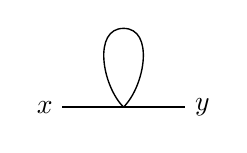
\begin{tikzpicture}
				\begin{feynhand}
					\vertex  (a) at(-1, 0) {$x$};
					\vertex  (b) at (1, 0) {$y$};
					\vertex (c) at (0, 0);
					\vertex (d) at (0, 1);
					\propag [plain] (a) to (b);
					\propag [plain] (c) to [out=45, in=0] (d) to [out=180, in=135] (c);
				\end{feynhand}
			\end{tikzpicture}
			=
			-\i\lambda\int \dd[4]{z} D(x-z)D(z-y)D(z_1-z_2) -\i\lambda\int \dd[4]{z} D(x-z)D(z-y)D(z_2-z_1)
		\end{equation}
		わかりやすさのために,まず区別して$z_1$と$z_2$としたが,これらは同じもので,重み$1$で足さなければいけないので,Symmetry factor $2$で割る必要がある.
	\item 他にも,統計力学っぽいところがあって,例えば,\textref{4.52}の和と積を入れ替える一連の計算は分配関数を計算するときによく使うテクニックである.
	\item \textref{4.55}の一つ前の式の右辺
		\begin{equation}
			\mel{\Omega}{\T(\phi(x)\phi(y))}{\Omega}\lim_{T\to\infty(1-\i\varepsilon)}(\abs{\braket{0}{\Omega}}^2e^{-\i E_0 2T})
		\end{equation}
		について,$\mel{\Omega}{\T(\phi(x)\phi(y))}{\Omega} $は外点につながっているdiagramの和で,$\e^{-\i E_0 2T}$は真空泡と議論があるが,忘れ去られている
		$\abs{\braket{0}{\Omega}}^2$は\textref{4.55}の比例に吸収させると思う.
	\item \textref{4.58}は今まで浸かっていた``disconnected''というワードは外点にdisconnectedの意味で使われていたが,
		このように二つに別れてしまうdiagramのこともdisconnectedというので,注意が必要であることをいう.
		前者は以前の議論で,分母分子でキャンセルするのでcorrelation functionに寄与しないのに対し,後者は
		correlation functionに寄与するという違いがある.
	\item \textref{4.64}は,不安定状態を考えているので,$p^0\neq E_{\vec{p}}=\sqrt{\vec{p}^2 + m^2}$であることに注意して,
		\begin{align}
			\frac{1}{p^2-m^2 + \i m\Gamma}
			& = \frac{1}{(p^0)^2 - E_{\vec{p}}^2  +\i m\Gamma}\\
			& \sim \frac{1}{2E_{\vec{p}}(p^0-E_{\vec{p}}) + \i m\Gamma}\label{eq:on-shell_approx}\\
			& = \frac{1}{2E_{\vec{p}}(p^0-E_{\vec{p}}+\i m\Gamma/(2E_{\vec{p}}))}
		\end{align}
		となる.Eq. \eqref{eq:on-shell_approx}では
		$p^0$が$E_{\vec{p}}$に近いとしている.
	\item Peskinのin, out stateは相互作用場で$T\to \pm\infty$にしたと定義されているが,
		他の本\cite{Kugo1989}, \cite{Sakamoto2020}では$T\to\pm \infty$で自由場と一致しているとして,定めているので,in, out場の定義が違うので,注意が必要である.あとで,相互作用場での$\ket{\vec{p}}$を自由場での$\ket{\vec{p}}_0$で表す操作をするが,そちらが通常のin, out場の定義である.
	\item \textref{4.68}のimpact parameterによるphaseのずれだが,通常の平行移動とおもうと,指数の方はプラスで出るように思う.
		しかし,$k_{\mathcal{B}}$の全空間で積分しているし,これは先の計算でデルタ関数として現れるだけなので,
		あまり議論に影響はしない.

	\item \textref{4.70}のS-matrixの定義は,二行目から見るのがわかりやすくて,同じ時間$t=0$で$\ket*{\vec{k}_{\mathcal{A}}\vec{k}_{\mathcal{B}}}$と$\bra{\vec{p}_1\vec{p}_2\cdots}$があって,
		$\ket*{\vec{k}_{\mathcal{A}}\vec{k}_{\mathcal{B}}}$を$H$で$-T$時間発展させたのがin stateで
		$\bra{\vec{p}_1\vec{p}_2\cdots}$を$T$時間発展させたのがout stateである.
	\item S-matrixを考えれば良いのだが,常に存在する自明な項があるので,この本ではそれを除いて考える.
		常に出てくる項とは
		\begin{enumerate}
			\item $\mathsf{S} = 1 + \i \mathsf{T}$
				\footnote{$\mathsf{S}$をscattering matrix, $\mathsf{T}$をtransfer matrixと言う.日本語ではそれぞれ散乱行列と転送行列であり,その$\mathsf{S}$と$\mathsf{T}$であるとゼミでボケようと思ったが,それまでに炎上したので自粛した.余裕のある人はこのネタを供養してください.}
				と分けたときの,$1$
			\item 運動量保存の$(2\pi)^4\delta^{(4)}(p_{\mathcal{A}}+p_{\mathcal{B}} - \sum_fp_f)$\footnote{out stateの添字に$f$を使っているのは,final stateのfだと思う.}
		\end{enumerate}
		である.これらを除いたものがinvariant matrix element $\M$である.
	\item \textref{4.74}は運動量状態$\prod_f 1/\sqrt{2E_f}\ket{\vec{p}_1\cdots}$へのamplitudeを求めている.
		なぜ,\textref{4.68}の$\phi_f(\vec{p}_f)$などがないのかと悩んだが,これは波束をFourier変換したときの
		展開係数なので単なる一つのモードを考えている今は当然必要ない.
		また,$1/\sqrt{2E_f}$はLorentz不変なnormalizationのためのfactorで,求めたいのは確率なので,二乗すると,必要な式を得る.
	\item \textref{4.76}の$\dd{\sigma}$を求める計算は,まず$\bar{k}_i$の6つの積分をまず計算することで,barのついている変数がデルタ関数で潰れることを確認する.
		
		まず,ここではimplicitにビーム方向に$z$軸をとって,impact parameter方向の二次元を$\perp$と取っている.ここで,$\bar{k}_{\mathcal{B}}^{\perp}$積分で$\bar{k}_{\mathcal{B}}^{\perp} = k_{\mathcal{B}}^{\perp}$を得て,
		これと,前のデルタ関数の結果を先取りすることで,$\bar{k}_{\mathcal{A}}^{\perp} = \sum_fp_f^{\perp} - k_{\mathcal{B}}^{\perp} = k_{\mathcal{A}}$となる.

		z成分は\textref{4.77}の計算が必要だが,ここで使っているデルタ関数の公式は
		\begin{equation}
			\delta(f(x)) = \sum_{\text{zeros}}\frac{1}{\abs{f'(x)}}\delta(x-x_0)
		\end{equation}
		と全ての零点を拾わなければならないが,ここでは和がない.
		デルタ関数のなかにある$\bar{k}_{\mathcal{A}}^z$についての関数の零点は,一般に2つあることが予期されるので正確にはこれではいけないはずである.

		これは次のように解釈できる.今の状況は運動量が狭い範囲にある波束を考えているので,
		その範囲は零点を一つしか拾わないように設定されていると思う.
		実際,次の計算でそのような近似を使うので,そこまでは和の状況で残しておき,そこでひとつだけ零点を拾うという議論のほうが筋は良い気がする.

		今の積分は$\delta(\bar{E}_{\mathcal{A}} + \bar{E}_{\mathcal{B}}-\sum_fE_f)$で$\bar{k}_{\mathcal{A}}^z = \sum_fp_f^z - \bar{k}_{\mathcal{B}}^z$となっているものを計算していて,
		\begin{align}
			&\sqrt{(k_{\mathcal{A}}^{\perp})^2+(\textcolor{red}{\bar{k}_{\mathcal{A}}^z})^2+m_{\mathcal{A}}^2} + \sqrt{(k_{\mathcal{B}}^{\perp})^2 + (\sum_fp_f^z-\textcolor{red}{\bar{k}_{\mathcal{A}}^z})^2+m_{\mathcal{B}}^2}\\
			& = \sum_fE_f = E_{\mathcal{A}} + E_{\mathcal{B}}\\
			& = \sqrt{(k_{\mathcal{A}}^{\perp})^2+(\textcolor{red}{k_{\mathcal{A}}^z})^2+m_{\mathcal{A}}^2} + \sqrt{(k_{\mathcal{B}}^{\perp})^2 + (\sum_fp_f^z-\textcolor{red}{k_{\mathcal{A}}^z})^2+m_{\mathcal{B}}^2}
		\end{align}
		であるので,$\bar{k}_{\mathcal{A}}^z = k_{\mathcal{A}}^z$となり,
		$\bar{k}_{\mathcal{B}}^z = \sum_fp_f^z-k_{\mathcal{A}}^z = k_{\mathcal{B}}^z$となる.
		これで,$\vec{\bar{k}}_{i}^z = \vec{k}_i^z$が言えるので,エネルギーについても$\bar{E}_i=E_i$となり,
		\textref{4.78}のように二乗でまとめることができる.
	\item $k/E = v$の書き換えは,静止系からLorentz変換したことを考えると
		\begin{equation}
			\mqty(\gamma & \gamma\beta\\ \gamma\beta & \gamma)\mqty(m\\0) = \mqty(E\\k)
		\end{equation}
		なので,$k/E = \beta = v$となる.

	\item \textref{4.82}でもデルタ関数の公式を使って,$\delta(E_{\text{CM}}-E_1-E_2)=(p_1/E_1 + p_1/E_2)^{-1}\delta(p-p_0)$としているが,これも真面目に考えるとおかしくて,$p_1$積分は$0\to \infty$で零点を計算をするとプラスマイナスの組ででてくるので複数拾うことはないにしろ,$E_{\text{CM}} < m_1+m_2$だと解を持たないのでゼロになる.
		零点をしらべるより,デルタ関数を変数変換して調べたほうがわかりやすくて\cite{Schwartz:2014sze},$x\coloneqq \sqrt{p_1^2+m_1^2} + \sqrt{p_1^2 + m_2^2} - E_{\text{CM}}$すると,
		\begin{equation}
		\int_{m_1+m_2-E_{\text{CM}}}^{\infty}\delta(x)
		\end{equation}
		となるが,これは$m_1+m_2 > E_{\text{CM}}$だと$0$を拾わない.
		
		しかし,これは物理的に考えるとtotal energyがmassより小さかったら,そのような散乱は起こらず興味のない結果になってしまうので,これが満たされているのは当然とも思える.
	\item \textref{4.102}の$1/2$のfactorはloopのsymmetry factorで割っている.

	\item Fermionの一粒子状態を$\ket{\vec{p}, s}$と書いただけでは$(a_{\vec{p}}^s)^{\dagger}\ket{0}$のfermionか$(b_{\vec{p}}^s)\ket{0}$のantifermionか区別がつかない.
		これで良いのかと聞いたところ,そもそも実用的にはまずdiagramを直接書いて計算するので,この記法を使った縮約の式に戻ることは殆ど無いそうである\footnote{ただし,symmetry factorを調べるときはdiagramだけだと探し漏れがあるので,
		その場合は縮約の式に戻って調べるという使い方をするそう.}.ここは,教育的配慮と認識して,上手く解釈するのが吉.
	\item \textref{4.115}で
		\begin{equation}
			\wick{\langle \c5{\vec{p}'}, \c2{\vec{k}'}\rvert \c2{\bar{\psi}_x}\c3{\psi_x}\c1{\phi_x}\c5{\bar{\psi}_y}\c4{\psi_y}\c1{\phi_y}\lvert \c4{\vec{p}}, \c3{\vec{k}}\rangle} 
		\end{equation}
		の縮約で,$\bar{\psi}$が入れ替わっている箇所があるように思うが,p. 119で説明があるように$\bra*{\vec{p}', \vec{k}'} = \bra{0}a_{\vec{k}'}a_{\vec{p}'}$と外れるので,この計算はあっている.
		また,spinorの順番が$\bar{u}u\bar{u}u$になっているのは当然で,$u$は4成分あるので,この順番でないと1成分に縮約できない.
	\item \textref{4.130}の$\partial^2A_{\mu} = 0$のゲージのとり方をLorentz gaugeと書いてあるが,Lorenzである
		\footnote{日本語だと前者をローレンツ,後者をローレンスと表記することが多いと思う.}.
	\item Chapter 4.8の力の働き方が引力か斥力かという話は,\cite{Zee:2003mt}の一章にも経路積分形式で書かれている.
	\item \textref{4.132}は
		\begin{equation}
			\intp[4]{q}\frac{\i g_{\mu\nu}}{q^2+\i\epsilon}\e^{-\i q(x-y)}
			= \intp{q}(\i g_{\mu\nu})\e^{\i\vec{q}\cdot (\vec{x}-\vec{y})}\int\frac{\dd{q^0}}{2\pi} \frac{\e^{- \i q^0(x^0-y^0)}}{(q^0)^2-\abs{\vec{q}}^2 + \i\epsilon}
		\end{equation}
		として,後ろの計算を留数積分でする.

		\begin{equation}
			I  =\int \dd{z}\frac{\e^{-\i zx}}{z^2-z_0^2 + \i\epsilon}
		\end{equation}
		は$z = \pm\sqrt{z_0^2-\i\epsilon}$にsimple poleがあり,下半平面で積分路を閉じると収束するので,$z = \sqrt{z_0^2-\i\epsilon}\sim \abs{z_0}$の方のpoleを拾って,
		\begin{equation}
			I = -2\pi\i\frac{\e^{-\i zx}}{2z}
		\end{equation}
		なので教科書の結果を得る.
	\item \textref{4.133}の計算を縮約に戻ってやると次のようになる.
		\begin{align}
			&\i \M (2\pi)^4\delta^{(4)}(p+k -p'-k')
			\\&= 
			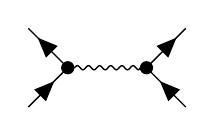
\begin{tikzpicture}[baseline=(x.base)]
				\begin{feynhand}
					\vertex [dot] (x) at (-0.5, 0) {};
					\vertex [dot] (y) at (0.5, 0) {};
					\vertex (p) at (-1, -0.5);
					\vertex (p') at (-1, 0.5);
					\vertex (k) at (1, -0.5);
					\vertex (k') at (1, 0.5);
					\propag[fermion] (p) to (x);
					\propag[fermion] (x) to (p');
					\propag[fermion] (k) to (y);
					\propag[fermion] (y) to (k');
					\propag[photon] (x) to (y);
				\end{feynhand}
			\end{tikzpicture}\\
			&= \bra{0}\wick{\c2{a_{k'}}\c4{a_{p'}}\qty(-\i e\int \dd[4]{x})\c4{\bar{\psi_x}}\gamma^{\mu}\c3{\psi_x}\c5{A_\mu}\qty(-\i e\int\dd[4]y)\c2{\bar{\psi_y}}\gamma^{\nu}\c1{\psi_y}\c5{A_\nu}\c3{a_p^{\dagger}}\c1{a_k^{\dagger}}}\ket{0}\\
			&= (-\i e)^2\int \dd[4]{x}\int \dd[4]{y}\bra{0}\wick{\c2{a_{k'}}\c4{a_{p'}}\c4{\bar{\psi_x}}(-1)\c2{\bar{\psi_y}}\gamma^{\mu}\c5{A_\mu}\gamma^{\nu}\c1{\psi_y}\c5{A_\nu}(-1)\c3{\psi_x}\c3{a_p^{\dagger}}\c1{a_k^{\dagger}}}\ket{0}\\
			&= (-\i e)^2\int\dd[4]{x}\int \dd[4]{y}\intp[4]{q}
			\bar{u}(p')\e^{\i p'x}\gamma^{\mu}u(p)\e^{-\i px}\frac{-\i g_{\mu\nu}}{q^2+\i\epsilon}\e^{-\i q(x-y)}\bar{u}(k')\e^{\i k'y}\gamma^{\nu}u(k)\e^{-\i kx}\\
			&= (-\i e)^2\intp[4]{q}\bar{u}(p')\gamma^{\mu}u(p)\frac{-\i g_{\mu\nu}}{q^2+\i\epsilon}\bar{u}(k')\gamma^{\nu}u(k)(2\pi)^4\delta^{(4)}(p+q-p')(2\pi)^4\delta^{(4)}(k-q-k')\\
			&= (-\i e)^2\bar{u}(p')\gamma^{\mu}u(p)\frac{-\i g_{\mu\nu}}{(p'-p)^2}\bar{u}(k')\gamma^{\nu}u(k) (2\pi)^4\delta^{(4)}(p+k-p'-k')
		\end{align}
		となり,常に出てくる外線の運動量保存を省いたものが\textref{4.133}である\footnote{もっと丁寧にやるべきところは,gamma行列とspinorのspinor添字をちゃんと書いて,行列の積の順序がこれで良いか確かめることである.}.

\end{itemize}

	\section{Elementary Process of Quantum Electrodynamics}
\begin{itemize}
	\item $\i\M = (\i\e^2/q^2)\bar{v}(p')\gamma^{\mu}u(p)\bar{u}(k)\gamma_{\mu}v(k')$だが,cross sectionを求める際は$\abs{\M}^2$が必要で,$(\bar{v}\gamma^{\mu}u)^{*}$が必要であるが,これはbarのnotationが優れているポイントで,
		$(\gamma^0)^{\top} = \gamma^{0}$, $(\gamma^{i})^{\top} =- \gamma^{i}$であるので,$(\bar{v}\gamma^{\mu}u)^{*} = \bar{u}\gamma^{\mu}v$である.
	\item p.132でspinの向きを指定せず平均をとる操作をするが,これは始状態の$\mathrm{e^+}$, $\mathrm{e^-}$に対してであり,終状態の$\mathrm{\mu^+}$, $\mathrm{\mu^-}$については和をとるので,$1/2$のfactorは$s$, $s'$についての和に関してかかり,\textref{5.4}では全体で$1/4$のfactorがかかる.
	\item \textref{5.4}での$\tr$はスピノル添字に関してのtraceであることに注意.$\mu$などはベクトルの添字なのでtraceには関係しない.
	\item $\tr\qty((\slashed{p} -m_{\elec})\gamma^{\mu}(\slashed{p}+m_{\elec}\gamma^{\nu})) = 4\qty((p')^\mu p^\nu + (p')^\nu p^\mu - g^{\mu\nu}(p\cdot p' + m_\elec^2))$
		は$\slashed{p} = \gamma^{\mu} p_\mu$に注意して,Gamma行列に対してのTraceの公式を使えば導ける.
	\item \textref{5.6}の等式はあとで使う.一番最後の$\epsilon^{\alpha\beta\mu\nu} \epsilon_{\alpha\beta\rho\sigma} = -2(\delta\indices{^\mu_\rho}\delta\indices{^\nu_\sigma} - \delta\indices{^\mu_\sigma}\delta\indices{^\nu_\rho})$から示す.

		まず,これはすでに$\alpha$, $\beta$に関して和を取られているので,$\mu$, $\nu$が$\alpha$, $\beta$と一致すると完全反対称性からゼロになる.つまり,$\mu$ ($\nu$)は$\rho$か$\sigma$と一致しなければならない.また,$\mu$と$\nu$, $\rho$と$\sigma$は反対称なので,反対称に組まなければいけない.
		これらから$\epsilon^{\alpha\beta\mu\nu} \epsilon_{\alpha\beta\rho\sigma} \propto \delta\indices{^\mu_\rho}\delta\indices{^\nu_\sigma} - \delta\indices{^\mu_\sigma}\delta\indices{^\nu_\rho}$である.
		
		比例定数$c$は$\mu$, $\nu$, $\rho$, $\sigma$に適当な文字を入れて決定すればよい.$(\mu, \nu) = (\rho, \sigma) = (2, 3)$として,
		$\epsilon^{0123}\epsilon_{0123}  + \epsilon^{1023}\epsilon_{1023} = -2$\footnote{$\epsilon^{0123} = 1$とする規約で,
		全ての添字を下ろすと,
		空間成分$1$, $2$, $3$を下ろすときに奇数回$-1$が出るので,
		$\epsilon_{0123} = -1$}.
		一方,$c(\delta\indices{^2_2}\delta{^3_3} - \delta{^2_3}\delta{^3_2}) = a$より$c = -2$であるので,主張は示された.
	\item \textref{5.7}の等式は$\gamma^{\mu}$の数$n$が偶数のとき成り立つ.
		奇数ならば,\textref{5.5}の二番目の式からゼロになる.
		$\gamma^5$が入った場合もなりたつと書いてあるが,$\gamma^{5}$の個数は$n$にカウントしないと思う.また,$\gamma^5$が入ったとき$n$が奇でもゼロになるとは言えない.例えば$n=4$のとき$\epsilon^{\mu\nu\rho\sigma}$に比例する.
\end{itemize}

	\section{Radiative correction}
\begin{itemize}
	 \item bremsstrahlungで出てくるphotonは低エネルギー過ぎて観測できないので,実験上は
	 \begin{center}
	 	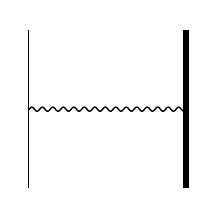
\begin{tikzpicture}
			\begin{feynhand}
				\vertex (a) at (-1, -1);
				\vertex (b) at (-1, 1);
				\vertex (c) at (1, -1);
				\vertex (d) at (1, 1);
				\propag[plain, line width=2pt] (c) to (d);
				\propag[plain] (a) to (b);

				\vertex (e) at (-1, 0);
				\vertex (f) at (1, 0);
				\propag[photon] (e) to (f);
			\end{feynhand}
		\end{tikzpicture}
		\qquad{}と\qquad{}
	 	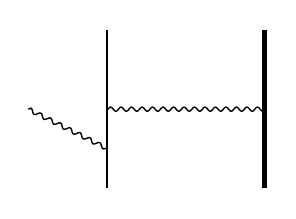
\begin{tikzpicture}
			\begin{feynhand}
				\vertex (a) at (-1, -1);
				\vertex (b) at (-1, 1);
				\vertex (c) at (1, -1);
				\vertex (d) at (1, 1);
				\propag[plain, line width=2pt] (c) to (d);
				\propag[plain] (a) to (b);

				\vertex (e) at (-1, 0);
				\vertex (f) at (1, 0);
				\propag[photon] (e) to (f);

				\vertex (h) at (-1, -0.5);
				\vertex (g) at (-2, 0);
				\propag[photon] (h) to (g);
			\end{feynhand}
		\end{tikzpicture}
	\end{center}
	は区別できないのだが,計算上はすべてのprocessを取り込む必要がある.
	masslessの粒子がいると,このようにいくらで低エネルギーのものをとりこんで,
	エネルギースペクトラムは$m_\elec$から上は連続的になる.

	\item \textref{6.1}以外にheavy particleを含むloop diagramが次の6種類ある.
	loop diagramとは,外線の運動量を決めても内線の運動量がuniqueに決まらないdiagramであることに注意.
	\begin{center}
		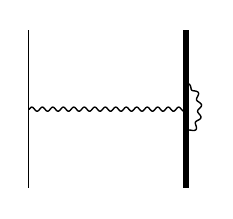
\begin{tikzpicture}
			\begin{feynhand}
				\vertex (a) at (-1, -1);
				\vertex (b) at (-1, 1);
				\vertex (c) at (1, -1);
				\vertex (d) at (1, 1);
				\propag[plain, line width=2pt] (c) to (d);
				\propag[plain] (a) to (b);

				\vertex (e) at (-1, 0);
				\vertex (f) at (1, 0);
				\propag[photon] (e) to (f);

				\vertex (h) at (1, -0.3);
				\vertex (g) at (1, 0.3);
				\propag[photon] (h) to  [out=0, in=0](g);
			\end{feynhand}
		\end{tikzpicture}
		,\quad
		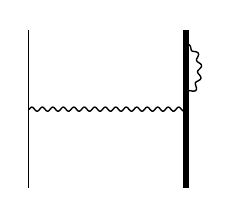
\begin{tikzpicture}
			\begin{feynhand}
				\vertex (a) at (-1, -1);
				\vertex (b) at (-1, 1);
				\vertex (c) at (1, -1);
				\vertex (d) at (1, 1);
				\propag[plain, line width=2pt] (c) to (d);
				\propag[plain] (a) to (b);

				\vertex (e) at (-1, 0);
				\vertex (f) at (1, 0);
				\propag[photon] (e) to (f);

				\vertex (h) at (1, 0.2);
				\vertex (g) at (1, 0.8);
				\propag[photon] (h) to [out=0, in=0](g);
			\end{feynhand}
		\end{tikzpicture}
		,\quad
		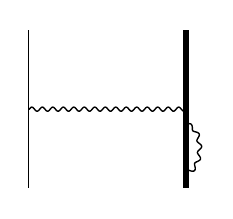
\begin{tikzpicture}
			\begin{feynhand}
				\vertex (a) at (-1, -1);
				\vertex (b) at (-1, 1);
				\vertex (c) at (1, -1);
				\vertex (d) at (1, 1);
				\propag[plain, line width=2pt] (c) to (d);
				\propag[plain] (a) to (b);

				\vertex (e) at (-1, 0);
				\vertex (f) at (1, 0);
				\propag[photon] (e) to (f);

				\vertex (h) at (1, -0.2);
				\vertex (g) at (1, -0.8);
				\propag[photon] (h) to [out=0, in=0] (g);
			\end{feynhand}
		\end{tikzpicture}
		, \quad
		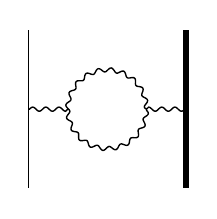
\begin{tikzpicture}
			\begin{feynhand}
				\vertex (a) at (-1, -1);
				\vertex (b) at (-1, 1);
				\vertex (c) at (1, -1);
				\vertex (d) at (1, 1);
				\propag[plain, line width=2pt] (c) to (d);
				\propag[plain] (a) to (b);

				\vertex (e) at (-1, 0);
				\vertex (f) at (-0.5, 0);
				\propag[photon] (e) to (f);

				\vertex (g) at (1, 0);
				\vertex (h) at (0.5, 0);
				\propag[photon] (g) to (h);
				\vertex (i) at (0, 0.5);
				\vertex (j) at (0, -0.5);
				\propag[photon] (h) to [out=270, in=0] (j) to [out=180, in=270] (f) to [out=90, in=180] (i) to [out=0, in=90] (h);
			\end{feynhand}
		\end{tikzpicture}
		,\quad
		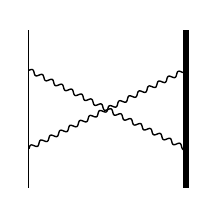
\begin{tikzpicture}
			\begin{feynhand}
				\vertex (a) at (-1, -1);
				\vertex (b) at (-1, 1);
				\vertex (c) at (1, -1);
				\vertex (d) at (1, 1);
				\propag[plain, line width=2pt] (c) to (d);
				\propag[plain] (a) to (b);

				\vertex (e) at (1, 0.5);
				\vertex (f) at (1, -0.5);
				\vertex (g) at (-1, 0.5);
				\vertex (h) at (-1, -0.5);

				\propag[photon] (g) to (f);
				\propag[photon] (h) to (e);
			\end{feynhand}
		\end{tikzpicture}
		, \quad
		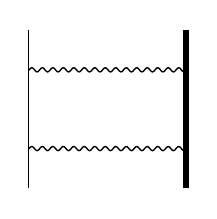
\begin{tikzpicture}
			\begin{feynhand}
				\vertex (a) at (-1, -1);
				\vertex (b) at (-1, 1);
				\vertex (c) at (1, -1);
				\vertex (d) at (1, 1);
				\propag[plain, line width=2pt] (c) to (d);
				\propag[plain] (a) to (b);

				\vertex (e) at (1, 0.5);
				\vertex (f) at (1, -0.5);
				\vertex (g) at (-1, 0.5);
				\vertex (h) at (-1, -0.5);

				\propag[photon] (g) to (e);
				\propag[photon] (h) to (f);
			\end{feynhand}
		\end{tikzpicture}
	\end{center}
	\item \textref{Fig. 7.2}などはmassless photonがいないと仮定して,スペクトラムを書いている.
	このときは図にあるように$2m_\elec$から状態が連続的に分布する.
	状態があると,相関関数のFourier変換がpoleを持つらしく,連続spectrumだと大体poleが連続的に分布すると思えば,そこにbranch cutが走ることになる.
	\end{itemize}




	\begin{itemize}
	\item \textref{6.4}では$m\epsilon$を改めて$\epsilon$とおいている.

	\item \textref{6.5}の計算で$1/k^2$のpoleを両方下に下げる遅延条件を設定することは,今$t=0$で瞬間的に加速されることを考えているので,それ以前に放射の場はなくて,その後には存在するという境界条件を課していることと思える
	\footnote{今,微分方程式をFourier変換したものを考えており,このようなpoleをずらす操作は適切な境界条件を与えていると思える.}.

	$t>0$の場合でも放射が起こるのか,と混乱したが,そうではなくて$t=0$の瞬間に放射が起こったものが$t>0$でも残っていると思うと教えてもらった.
	\item \textref{6.5}の$k^0$についての積分を行う際に,複素関数として,上(下)半平面に積分路を追加してそれがゼロに飛ぶことを使うが,
	$\e^{\i kz} = \e^{\i kR\cos\theta - kR\sin\theta}$をゼロに飛ばしたときに$\theta \sim 0$の範囲で本当に収束するのかという質問がでた.
	これは,一般論としては\href{https://ja.wikipedia.org/wiki/\%E3\%82\%B8\%E3\%83\%A7\%E3\%83\%AB\%E3\%83\%80\%E3\%83\%B3\%E3\%81\%AE\%E8\%A3\%9C\%E9\%A1\%8C}{Jordanの補題}というのがあって,その証明を追えばよいのだが,収束することは次のように言える.

	まず,積分について$f(z)$を$M/R^k$, $(k>0)$程度で抑えられる関数\footnote{たとえば$1/(k^2 + m^2)$なら$k=3$くらい,今の場合の$1/(k^4(k+m)(k-m))$だと$k=5$など.}として,
	\begin{align}
		\int \dd{z}f(z)e^{\i kz} &= \int_{0}^{\pi} \dd{\theta}\i R\e^{\i\theta} f(R\e^{\i\theta})\e^{\i kR\cos\theta - kR\sin\theta}\\
		&= 2\int_{0}^{\pi/2} \dd{\theta}\i R\e^{\i\theta} f(R\e^{\i\theta})\e^{\i kR\cos\theta - kR\sin\theta}\\
	\end{align}
	とできる.$\pi/2 \leq \theta \leq \pi$については$\theta \to \pi-\theta$としてまとめた.

	$0 \leq \theta \leq \pi/2$においては$\sin\theta \geq 2\theta/\pi$
	が成り立つので,
	\begin{align}
		\abs{\int_{0}^{\pi/2} \dd{\theta}\i R\e^{\i\theta} f(R\e^{\i\theta})\e^{\i kR\cos\theta - kR\sin\theta}}
		&\leq \int_{0}^{\pi/2}\dd{\theta}R\abs{f(R\e^{\i\theta})}\e^{-kR\sin\theta}\\
		&\leq \frac{M}{R^k}\int_{0}^{\pi/2}\dd{\theta}\e^{-kR2\theta/\pi}\\
		&= \frac{M}{R^k}\frac{\pi}{2kR}(1 - \e^{-kR})\\
		&\leq \frac{\pi}{2kR^k}M \underset{R\to\infty}{\to} 0
	\end{align}
	となる.
	\item p.178の一番下の式からp.179の最初の式で負号が消えているのは,$p^{\mu} = (p^0, \vec{0})$と設定したので,$k^0 = \vec{k}\cdot \vec{p}/p^0 = 0$だから,分母の$k^2 = -\abs*{\vec{k}}^2$の負号が出てくるからである.

	\item \textref{6.10}の絶対値はベクトルの絶対値で,\textref{6.8}で実数に設定しているので複素共役をとる必要はない.
	また,$1/8$の係数は,エネルギーの定義の$1/2$と$\R\ni a = (z+z^*)/2$と書くときの$1/2$のfactor 2つ分によりついている.

	\item \textref{6.10}の$\vec{B}$側の評価で,形は$\vec{E}$のほうと同じだから,
	\begin{equation}
		\frac{1}{2}\int\dd[3]{x}\abs*{\vec{B}(x)}^2
		= \frac{1}{8}\intp[3]{k}
		\qty(\vec{\mathcal{B}}(\vec{k})\cdot \vec{\mathcal{B}}(\vec{-k})\e^{-2\i k^0t}
		+ 2\vec{\mathcal{B}}(\vec{k}) \cdot \vec{\mathcal{B}}^{*}(\vec{k})
		+ \vec{\mathcal{B}}^{*}(\vec{k}) \cdot \vec{\mathcal{B}}^{*}(\vec{-k})\e^{2\i k^0t})
	\end{equation} 
	となる.
	ここで,ベクトル解析の式$(\vec{A}\times\vec{B})\cdot(\vec{C}\times \vec{D}) = (\vec{A}\cdot \vec{C})(\vec{B}\cdot \vec{D}) - (\vec{A}\cdot\vec{D})(\vec{B}\cdot \vec{C})$をつかい,$\vec{\mathcal{B}} = \hat{\vec{k}} \times \vec{\mathcal{E}}$であることと$\vec{k} \cdot \vec{\mathcal{E}} = 0$を考慮すると$\vec{\mathcal{B}}(\vec{k})\cdot\vec{\mathcal{B}}(-\vec{k}) = -\vec{\mathcal{E}}(\vec{k})\cdot\vec{\mathcal{E}}(-\vec{k})$などとなり,$\e^{\pm \i k^0t}$の項は足すと消える.

	\item 偏光ベクトル$\epsilon^{\mu}$は四元ベクトルだが,ゲージ対称性で一成分,zero normのunphysical stateを消すために一成分消えるので,独立なものは二つ.
	\item \textref{6.13}で$\sum \epsilon_\mu\epsilon_\nu^{*}$を$-g_{\mu\nu}$に置き換えてよいのは,$k_{\mu}(p'^{\mu}/(k\cdot p') - p^{\mu}/(k\cdot p)) = 0$がなりたつ.
	\textref{5.79}あたりの議論を追うと
	まず,$k^{\mu*} = (k, 0,0, k)$, $\epsilon^1 = (0, 1, 0, 0)$, $\epsilon^2 = (0, 0, 1, 0)$をとり,
	$k_{\mu}f^{\mu} = 0 $が成り立っている.$k$の取り方から,
	$kf^0 - kf^3 = 0$がわかり,
	$\sum \epsilon_\mu\epsilon_\nu f^\mu f^{\nu *} = \abs{f^1}^2 L \abs{f^2}^2 = \abs{f^1}^2 + \abs{f^2}^2 + \abs{f^3}^2 - \abs{f^0}^2 = g_{\mu\nu}f^{\mu}f^{\nu * }$となるので,
	この置き換えをしてよいことがわかる.(逆に,この種の条件がない場合は置き換えができない.)
	

	\item p.181最後に積分の下端を設定するところの$\vec{v}$などはhigh energyを考えているので$\abs*{\vec{v}} \sim 1$であることに今後注意すべき.
	また,この下端の設定は任意性があり,今考えているのは放射が軸にほぼ平行な$\cos\theta \sim 1$あたりからの寄与がdominantであるからである.

	この設定に物理的解釈をつけようと思うと,後ろに放射することはないだろうとおもい,方向転換する角度でcutoffするという説明を教えてもらった.


	\item \textref{6.17}の$\approx 2\log(p\cdot p'/((E^2-\abs*{\vec{p}})/2))$への変形は,分母の$E^2(E-\abs*{\vec{p}}) \simeq (E+\abs*{\vec{p}})/2(E-\abs*{\vec{p}})$と考えるとよい.
	また,直接しらべるとこの途中式を経ず,最後の形にもっていくこともできるらしい. 
	\item \textref{6.17}の最後は等号だが近似を使っている.
\end{itemize}

	\bibliography{QFT}
	\bibliographystyle{ytamsalpha}
	%\bibliographystyle{ytamsbeta}
\end{document}
